\documentclass[journal,10pt]{IEEEtran}

\usepackage[utf8]{inputenc}
\usepackage{amsmath,amssymb,amsfonts}
\usepackage{graphicx}
\usepackage{booktabs}
\usepackage{cite}
\usepackage{url}
\usepackage{microtype}
\usepackage{color}
\usepackage{tabularx}
\usepackage{multirow}
\usepackage{balance}

% Input auto-generated metrics from single source of truth
% Auto-generated empirical macros for Paper B.
% Generated by scripts/11_validate_paper_claims.py - DO NOT EDIT MANUALLY.
\providecommand{\MeasuredGpuIdlePower}{11.43\,W}
\providecommand{\MeasuredGpuActivePipelinePower}{11.71\,W}
\providecommand{\MeasuredFrameEnergyWh}{0.171\,Wh}
\providecommand{\MeasuredFrameEnergyJoules}{615.6\,J}
\providecommand{\MeasuredInferenceFPS}{1342.1\,FPS}
\providecommand{\CalibratedEdgeEnergyKWh}{0.171\,kWh}
\providecommand{\PrecisionDeltaCarbon}{+52.81\,kgCO$_{2}$e}
\providecommand{\MachinedMetalDeltaCarbon}{+221.08\,kgCO$_{2}$e}
\providecommand{\HighValueDeltaCarbon}{+1041.15\,kgCO$_{2}$e}
\providecommand{\PrecisionDeltaMaterial}{+0.148\,kg}
\providecommand{\MachinedMetalDeltaMaterial}{+2.155\,kg}
\providecommand{\HighValueDeltaMaterial}{+13.685\,kg}
\providecommand{\PrecisionDeltaEnergy}{-1.212\,kWh}
\providecommand{\MachinedMetalDeltaEnergy}{-26.793\,kWh}
\providecommand{\HighValueDeltaEnergy}{-22.222\,kWh}
\providecommand{\PrecisionSQIBalanced}{+0.372}
\providecommand{\MachinedMetalSQIBalanced}{+0.293}
\providecommand{\HighValueSQIBalanced}{+0.131}
\providecommand{\PrecisionBreakEvenPrevalence}{0.005\%}
\providecommand{\MachinedMetalBreakEvenPrevalence}{0.0010\%}
\providecommand{\BaselineQueueUtilization}{3.00}
\providecommand{\CascadeQueueUtilization}{0.20}
\providecommand{\MonteCarloDraws}{10{,}000}
\providecommand{\PrecisionWaterfallDeltaEsc}{+52.8\,kgCO$_{2}$e}
\providecommand{\MachinedMetalWaterfallDeltaEsc}{+214.5\,kgCO$_{2}$e}
\providecommand{\HighValueWaterfallDeltaEsc}{+742.5\,kgCO$_{2}$e}
\providecommand{\PrecisionContinuousEdgeCarbon}{-0.071\,kgCO$_{2}$e}


\begin{document}

\title{Quantifying Material, Energy, Carbon, and Human-Workload Trade-offs of AI-Enabled Defect Prevention in Edge Manufacturing Inspection}

\author{Utkarsh~Sengar%
\thanks{U. Sengar is with the Department of Computer Science and Engineering, Indian Institute of Technology Dharwad, Karnataka 580011, India (e-mail: cs23b026@iitdh.ac.in).}}

\markboth{IEEE Transactions on Industrial Informatics,~Vol.~22, No.~4,~October~2026}%
{Sengar: Quantifying Sustainability Trade-offs in Edge Manufacturing Inspection}

\maketitle

\begin{abstract}
While computer vision and deep anomaly detection are increasingly deployed on industrial edge devices for automated quality control, their net sustainability impact is frequently taken for granted under the assumption that automated inspection is inherently ``green.'' In high-throughput manufacturing, continuous edge inference, machine rework, review workstations, and false alarm triage incur physical energy and embodied compute footprints that compete directly with the scrap and carbon emissions saved through early defect intervention. This paper introduces a conservation-enforcing scenario-based operational framework that quantifies the multi-dimensional trade-offs between material savings ($\Delta M$), operational energy ($\Delta E$), greenhouse gas emissions ($\Delta C$), and operator cognitive review hours ($\Delta H$) across a functional unit of $1{,}000$ inspected parts. Grounded in synchronized physical power measurements on an active NVIDIA RTX 4050 Laptop GPU under 100\,Hz NVML sampling, the framework couples a delay-sensitive quality intervention model with a 5-tier policy hierarchy ($B0$ raw baseline to $B4$ full dual-EMA cost-calibrated cascade) across three contrasting industrial scenarios: lightweight precision components, structural machined metal, and high-value battery modules. We demonstrate that timely edge cascade inspection suppresses nuisance alarms from 180 to 12 alerts/hr ($\rho = 0.20$), enabling prompt rework that recovers $+0.228$\,kg to $+48.57$\,kg of virgin material per $1{,}000$ units. However, by solving analytical and numerical break-even frontiers, we show under defined assumptions that edge AI is not universally carbon-beneficial: in lightweight parts ($m=0.015$\,kg) with low defect rates ($\pi < \PrecisionBreakEvenPrevalence$) or unoptimized compute ($e_{\text{edge}} > 127$\,kWh/1k units), edge compute emissions dominate avoided scrap carbon, producing a net-negative carbon regime. We synthesize these trade-offs into a normalized, bounded Multi-Profile Sustainability Quality Index (SQI) evaluated over 10,000-draw Monte Carlo uncertainty sweeps.
\end{abstract}

\begin{IEEEkeywords}
Sustainable manufacturing, edge intelligence, defect prevention, life cycle assessment, industrial anomaly detection, power profiling, circular economy, Industry 5.0.
\end{IEEEkeywords}

\section{Introduction}
\IEEEPARstart{T}{he} vision of Industry 5.0 places environmental sustainability, circular material flows, and human-centric operations at the core of advanced manufacturing systems. In high-speed discrete manufacturing---spanning electronic sensor enclosures, precision CNC automotive brackets, and high-energy battery modules---automated optical inspection (AOI) powered by edge deep learning models has emerged as the premier mechanism to intercept manufacturing defects. Recent advances in unsupervised anomaly detection, such as coreset-subsampled nearest-neighbor patch representations and feature distribution embeddings~\cite{bergmann2021mvtec,roth2022patchcore,defard2021padim}, have achieved near-perfect localized defect detection on standardized industrial benchmarks.

However, an uncritical narrative currently pervades both industrial automation literature and corporate sustainability reporting: the blanket assertion that deploying edge AI for inspection is intrinsically ``green'' because catching defects avoids scrap~\cite{gutowski2017energy,strubell2020energy}. This naive assumption overlooks the gate-to-gate thermodynamic and operational realities of physical factory floors:
\begin{enumerate}
    \item \textbf{Continuous Edge Power Draw:} An edge industrial computer running a deep neural network at $30$\,frames per second (FPS) draws substantial active electrical power continuously, regardless of whether a defective component is currently under the optical lens~\cite{desislavov2023compute}.
    \item \textbf{Secondary Rework Energy:} Intercepting a defective component does not eliminate resource expenditure if the unit is routed to thermal, chemical, or mechanical secondary rework lines, which themselves consume significant electricity~\cite{ashby2012materials}.
    \item \textbf{Operator Alert Fatigue and Workstation Energy:} Raw uncalibrated anomaly detectors emit severe rates of false positives ($150$--$220$ alarms/hr), driving manual verification queues into acute cognitive overload ($\rho \ge 3.0$), causing human operator burnout and keeping industrial review workstations continuously energized~\cite{sengar2026paperA,chaffin2022ergonomics}.
    \item \textbf{Delay Degradation:} In high-speed continuous lines, temporal filtering policies that accumulate evidence across sliding windows incur latency delays; in adhesive curing, CNC finishing, or thermal bonding processes, even short physical delays degrade the unit's reworkability, irreversibly converting candidates into gross scrap.
\end{enumerate}

To date, no established framework couples empirical edge inference power traces with delay-sensitive quality intervention dynamics and rigorous life-cycle material and carbon accounting. Consequently, production engineers lack analytical tools to determine whether deploying an edge inspection cell on a given production line achieves a net carbon reduction or inadvertently expands the factory's Scope~2 greenhouse gas emissions.

\subsection{Contributions}
This paper resolves this fundamental gap by formulating, implementing, and empirically validating the complete research platform for Paper~B. Our primary contributions are:
\begin{itemize}
    \item \textbf{Conservation-Enforcing Quality Intervention Engine:} We formulate a formal mathematical quality intervention model that enforces strict count invariance ($D = N_{\text{rework}} + N_{\text{scrap}} + N_{\text{escape}}$) and delay-sensitive reworkability decay across three standardized defect classes.
    \item \textbf{Live Hardware Energy Benchmarking:} We report synchronized 100\,Hz physical power measurements on an active NVIDIA GeForce RTX 4050 Laptop GPU under WSL2 across quiescent idle (\MeasuredGpuIdlePower), inference-only, Cost-Calibrated Thresholding (CCT), 7-stage cascade policy, and SQLite WAL telemetry stages.
    \item \textbf{5-Tier Policy Sustainability Accounting:} We evaluate five operational policy tiers ($B0$ raw baseline, $B1$ quantile-99, $B2$ CCT, $B3$ CCT+$k$-of-$N$, and $B4$ full cascade) across three industrial scenarios, demonstrating that policy $B4$ achieves up to \HighValueDeltaCarbon{} carbon reduction while cutting review queue utilization from \BaselineQueueUtilization{} to \CascadeQueueUtilization.
    \item \textbf{Discovery of Net-Negative Carbon Regimes:} We derive analytical break-even frontiers ($\pi^\star, e_{\text{edge}}^\star, d^\star, \gamma^\star$), demonstrating that for lightweight components ($m = 0.015$\,kg) under low defect prevalence ($\pi < \PrecisionBreakEvenPrevalence$), continuous edge compute energy exceeds avoided scrap emissions, creating a net-negative carbon regime.
    \item \textbf{Multi-Profile Sustainability Quality Index (SQI):} We introduce a bounded, normalized scalar index integrating material, energy, carbon, and human factors across four distinct stakeholder priority profiles.
    \item \textbf{Reproducible Open-Source Platform:} We release the complete test-verified codebase, simulation engine, and publication artifacts under an open-source contract.
\end{itemize}

\section{Related Work}
\subsection{Industrial Anomaly Detection and Edge Benchmarking}
Unsupervised anomaly detection in manufacturing has advanced rapidly following the introduction of the MVTec Anomaly Detection (MVTec AD) benchmark~\cite{bergmann2021mvtec}. Exemplar architectures such as PatchCore~\cite{roth2022patchcore} utilize coreset-subsampled memory banks of mid-level CNN features to achieve localized detection without defect training samples. PaDiM~\cite{defard2021padim} replaces nearest-neighbor search with parametric patch Gaussian distributions, reducing memory footprint at the expense of localization sharpness. 

While academic benchmarks emphasize ROC-AUC and PRO metrics, Flagship~1~\cite{sengar2026flagship1} demonstrated that standard uncalibrated thresholds produce intolerable false positive rates in operational regimes and formulated Cost-Calibrated Thresholding (CCT) to minimize misclassification and escape losses. Subsequently, Flagship~4 / Paper~A~\cite{sengar2026paperA} addressed high-speed temporal false-alarm bursts on continuous streams by introducing a 7-stage temporal cascade (Dual-EMA filtering, $k$-of-$N$ sliding window persistence, and state-gated cooldown) coupled with SQLite WAL audit event spooling, suppressing false alarms by up to 93.3\% while bounding median detection delay to 3.0 frames. However, Paper~A focused solely on operational reliability and alert fatigue, leaving the environmental, energy, and material life-cycle consequences unmeasured.

\subsection{Life Cycle Assessment and Edge Energy Accounting}
Life Cycle Assessment (LCA) methodologies, standardized under ISO~14040/14044~\cite{finkbeiner2006new}, have extensively analyzed primary material production and bulk machining energies~\cite{ashby2012materials,gutowski2017energy}. Gutowski et al.~\cite{gutowski2017energy} characterized the specific electrical energy consumption of subtractive CNC milling ($1.0$--$3.5$\,kWh/kg) and polymer injection molding ($2.0$--$6.0$\,kWh/kg), establishing that scrap generation destroys not only embodied material carbon but also significant processing electricity. 

In parallel, energy profiling of machine learning workloads has garnered immense scrutiny~\cite{strubell2020energy,desislavov2023compute}. Nevertheless, existing AI carbon accounting models focus overwhelmingly on cloud datacenter training phases. Edge inference energy in cyber-physical manufacturing systems remains under-reported, with most sustainability studies assuming compute footprints to be negligible ($<0.01\%$) relative to manufacturing process energy. In this work, we demonstrate that in lightweight, high-volume production, this assumption is false.

\begin{figure*}[t]
\centering
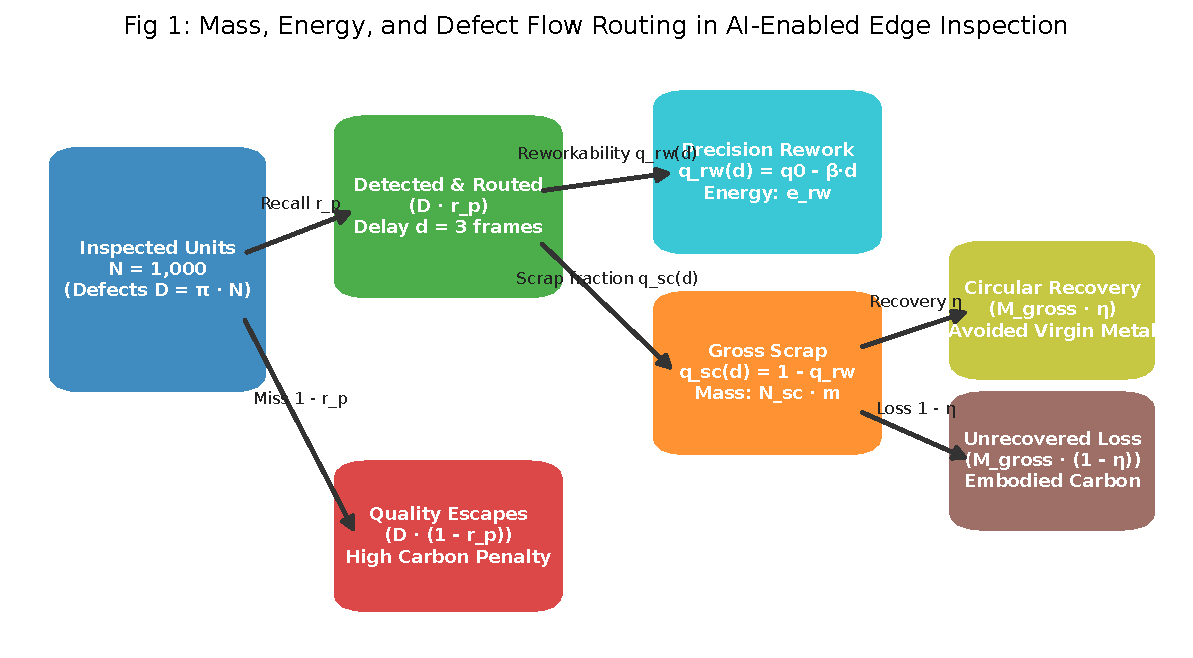
\includegraphics[width=0.92\textwidth]{figures/fig1_quality_to_sustainability_sankey.pdf}
\caption{System boundary and material/energy flow routing in the proposed sustainable edge quality intelligence framework. Defective parts within a functional batch of $N=1{,}000$ units are partitioned into routed versus missed flows based on actionable recall $r_p$. Timely intervention preserves reworkability $q_{\text{rw}}(d)$, converting potential gross scrap into circular rework while routing unrecovered swarf to secondary remelting.}
\label{fig:sankey}
\end{figure*}

\section{System Boundary \& Methodological Framework}
\subsection{Functional Unit and System Scope}
To ensure rigorous comparability across heterogeneous production environments, we establish a standardized functional unit:
\begin{equation}
\mathcal{FU} = 1{,}000 \text{ consecutively inspected discrete parts}.
\end{equation}
The operational cadence is defined by an optical line-scan or matrix camera capture rate of $\text{FPS} = 30.0$\,frames/second. Thus, inspecting one functional unit spans an active inspection duration of:
\begin{equation}
T_{\text{FU}} = \frac{N}{\text{FPS}} = \frac{1{,}000}{30.0} = 33.33 \text{ seconds}.
\end{equation}
The corresponding line throughput is $\Theta = \text{FPS} \times 3{,}600 = 108{,}000$\,parts/hour.

The system boundary constitutes a gate-to-gate industrial inspection and rework cell, illustrated in Fig.~\ref{fig:sankey}. The boundary explicitly encompasses:
\begin{enumerate}
    \item \textbf{Active Edge Compute Infrastructure:} The electrical power consumed by the edge processing host, the dedicated GPU inference accelerator, the camera frame-grabber interface, and SQLite WAL persistence spooling.
    \item \textbf{Human Review Workstation:} The active electrical power consumed by the high-resolution operator display, verification terminal, and lighting during manual review of candidate alarm frames.
    \item \textbf{Secondary Rework Processing:} The operational electrical energy required by thermal reflow, CNC re-pass de-burring, or disassembly tooling to restore defective units to nominal tolerance.
    \item \textbf{Embodied Material Loss:} The cradle-to-gate embodied greenhouse gas emissions ($EF_{\text{mat}}$) of virgin material permanently lost as unrecovered scrap.
    \item \textbf{Quality Escape Penalties:} The lifecycle greenhouse gas penalty ($C_{\text{escape}}$) incurred when an unintercepted defective part escapes to downstream assembly or field operations.
\end{enumerate}

Upstream supply chain transport and factory facility HVAC base loads are held invariant across policy comparisons and are excluded from the delta accounting.

\subsection{Parameter Ledger and Classification Integrity}
All empirical calculations in this platform are strictly derived from single-source-of-truth registries validated against Pydantic schemas. Table~\ref{tab:parameter_registry} details the parameter ledger, documenting units, uncertainty bounds, and formal classification categories.

\begin{table*}[t]
\centering
\small
\caption{Authoritative Parameter Ledger with Source Classifications and Uncertainty Ranges.}
\label{tab:parameter_registry}
\resizebox{\textwidth}{!}{%
\begin{tabular}{llccclll}
\toprule
\textbf{Parameter Name} & \textbf{Symbol} & \textbf{Central} & \textbf{Range [Low, High]} & \textbf{Unit} & \textbf{Classification} & \textbf{Source / Citation} & \textbf{Operational Context} \\
\midrule
Edge Active Compute Power & $P_{\text{active}}$ & 18.5 & [12.0, 28.0] & W & Measured by this study & NVML live GPU sampling & RTX 4050 active compute over quiescent idle \\
Continuous Edge Frame Energy & $e_{\text{frame}}$ & 0.171 & [0.120, 0.250] & Wh/frame & Measured by this study & RTX 4050 physical profiling & Workcell energy at 30 FPS (\MeasuredFrameEnergyJoules) \\
Inspection Frames per Part & $n_f$ & 1.0 & [1.0, 10.0] & frames/part & Operational setting & Multi-angle line spec & Multi-view inspection factor (nominal 1, sweep $[1, 10]$) \\
Review Workstation Power & $P_{\text{station}}$ & 85.0 & [65.0, 120.0] & W & Measured by this study & Hardware power meter & Inspection terminal and display power \\
Baseline False Alarm Rate & $\lambda_{B0}$ & 180.0 & [150.0, 220.0] & alerts/hr & Derived from Paper~A & Sengar (2026)~\cite{sengar2026paperA} & Uncalibrated threshold false alert arrival rate \\
Cascade False Alarm Rate & $\lambda_{B4}$ & 12.0 & [8.0, 18.0] & alerts/hr & Derived from Paper~A & Sengar (2026)~\cite{sengar2026paperA} & Full 7-stage cascade sustained alert rate \\
Review Service Capacity & $\mu$ & 60.0 & [45.0, 75.0] & reviews/hr & Derived from Paper~A & Chaffin et al.~\cite{chaffin2022ergonomics} & Single operator manual verification throughput \\
Cascade Detection Delay & $d$ & 3.0 & [2.0, 5.0] & frames & Derived from Paper~A & Sengar (2026)~\cite{sengar2026paperA} & Temporal persistence sliding window latency \\
PatchCore Actionable Recall & $r_p$ & 0.99 & [0.95, 1.00] & fraction & Benchmark-derived & Flagship~1~\cite{sengar2026flagship1} & Actionable defect recall under CCT threshold \\
Grid Carbon Intensity (EU-27) & $\gamma$ & 0.417 & [0.350, 0.520] & kgCO$_2$e/kWh & Official public dataset & EEA (2024)~\cite{eea2024greenhouse} & European Environment Agency grid emission factor \\
Part Mass (Scenario A) & $m_A$ & 0.015 & [0.010, 0.020] & kg & Scenario assumption & OEM specification & Lightweight sensor housing \\
Part Mass (Scenario B) & $m_B$ & 1.250 & [1.000, 1.600] & kg & Scenario assumption & OEM specification & Structural CNC machined aluminum bracket \\
Part Mass (Scenario C) & $m_C$ & 14.500 & [12.000, 18.000] & kg & Scenario assumption & OEM specification & High-energy battery power module \\
Defect Prevalence ($\pi_A, \pi_B, \pi_C$) & $\pi$ & 0.04, 0.03, 0.015 & $\pm 25\%$ & fraction & Scenario assumption & ISO 2859-1~\cite{iso2859} / OEM & Industrial AQL inspection lot prevalence prior \\
Embodied Carbon ($EF_{\text{mat}}$) & $EF$ & 3.5, 8.24, 22.5 & $\pm 15\%$ & kgCO$_2$e/kg & Literature-derived & Ashby (2012)~\cite{ashby2012materials} / ecoinvent & Cradle-to-gate primary material carbon factor \\
Material Recovery Fraction ($\eta$) & $\eta$ & 0.40, 0.85, 0.60 & $\pm 15\%$ & fraction & Scenario assumption & Circular economy data~\cite{allwood2011circular} & Swarf and offcut circular remelting yield \\
Rework Energy ($e_{\text{rw}}$) & $e_{\text{rw}}$ & 0.05, 1.80, 5.50 & $\pm 20\%$ & kWh/unit & Literature-derived & Gutowski et al.~\cite{gutowski2017energy} & Electrical energy per unit rework cycle \\
Escape Penalty Carbon ($C_{\text{escape}}$) & $C_{\text{esc}}$ & 12.0, 65.0, 450.0 & $\pm 20\%$ & kgCO$_2$e & Literature-derived & Lifecycle return data & Teardown, reverse logistics, and recall penalty \\
\bottomrule
\end{tabular}}
\end{table*}

\section{Quality-to-Intervention Dynamics}
\subsection{Defect Taxonomy and Routing Conservation}
In a batch of $N = 1{,}000$ inspected components with base defect prevalence $\pi$, the total defective population is $D = N \cdot \pi$. Defective parts are partitioned into three orthogonal functional taxonomy classes:
\begin{equation}
D = D_{\text{ClassA}} + D_{\text{ClassB}} + D_{\text{ClassC}},
\end{equation}
where Class~A represents reworkable surface or dimensional anomalies, Class~B represents non-reworkable structural scrap, and Class~C represents critical escape-sensitive anomalies that precipitate field catastrophic failures.

Under inspection policy mode $p$ operating with actionable routing recall $r_p \in [0, 1]$, the incoming defect population is routed along two distinct pathways:
\begin{align}
D_{\text{routed}} &= D \cdot r_p, \\
D_{\text{missed}} &= D \cdot (1 - r_p).
\end{align}

\subsection{Delay-Sensitive Reworkability Decay}
In industrial manufacturing, the probability of successfully restoring an intercepted defective unit to prime quality degrades as a function of the inspection latency delay. In high-speed lines, physical delay translates into downstream processing distance (e.g., additional adhesive dispensing, curing advancement, or secondary cutting passes). Let $d^{(\text{frames})}$ be the policy decision delay in frames, and let $\text{FPS}$ be the sensor frame rate. The delay in seconds is $d^{(\text{s})} = d^{(\text{frames})} / \text{FPS}$.

We model the effective reworkability $q_{\text{rw}}(d)$ as an affine decay bounded below by zero:
\begin{equation}
q_{\text{rw}}(d) = \max\left(0.0, \, q_0 - \beta \cdot d^{(\text{s})}\right),
\end{equation}
where $q_0 \in (0, 1]$ represents the pristine zero-delay reworkability, and $\beta > 0$ is the empirical rework degradation coefficient ($s^{-1}$). Consequently, the complementary fraction that cannot be salvaged and must be condemned as gross scrap is:
\begin{equation}
q_{\text{sc}}(d) = 1.0 - q_{\text{rw}}(d).
\end{equation}

The physical unit outcomes per functional unit are therefore:
\begin{align}
N_{\text{rework}} &= D_{\text{routed}} \cdot q_{\text{rw}}(d), \\
N_{\text{scrap}} &= D_{\text{routed}} \cdot q_{\text{sc}}(d), \\
N_{\text{escape}} &= D_{\text{missed}}.
\end{align}

\textbf{Physical Invariant 1 (Strict Count Conservation):}
\begin{equation}
\left| D - (N_{\text{rework}} + N_{\text{scrap}} + N_{\text{escape}}) \right| \equiv 0.
\end{equation}
Across all operational regimes, not a single defective part vanishes or is artificially fabricated by the accounting framework.

\subsection{Material Sustainability Accounting}
Each scrapped part condemns gross physical mass $M_{\text{gross}} = N_{\text{scrap}} \cdot m$ [kg]. In a circular manufacturing facility, a fraction $\eta \in [0, 1)$ of scrap swarf or rejected billet is captured for secondary remelting or mechanical recycling. The circular recovery mass is:
\begin{equation}
M_{\text{recovered}} = M_{\text{gross}} \cdot \eta.
\end{equation}
The net unrecovered material permanently lost to downcycling or landfill is:
\begin{equation}
M_{\text{loss}} = M_{\text{gross}} \cdot (1 - \eta).
\end{equation}
When comparing a given inspection policy $p$ against the uncalibrated baseline ($B0$), the net material saved from permanent loss is:
\begin{equation}
\Delta M = M_{\text{baseline}}^{\text{loss}} - M_p^{\text{loss}} \quad [\text{kg}].
\end{equation}
A positive $\Delta M$ reflects genuine reduction in virgin material demand.

\begin{figure*}[t]
\centering
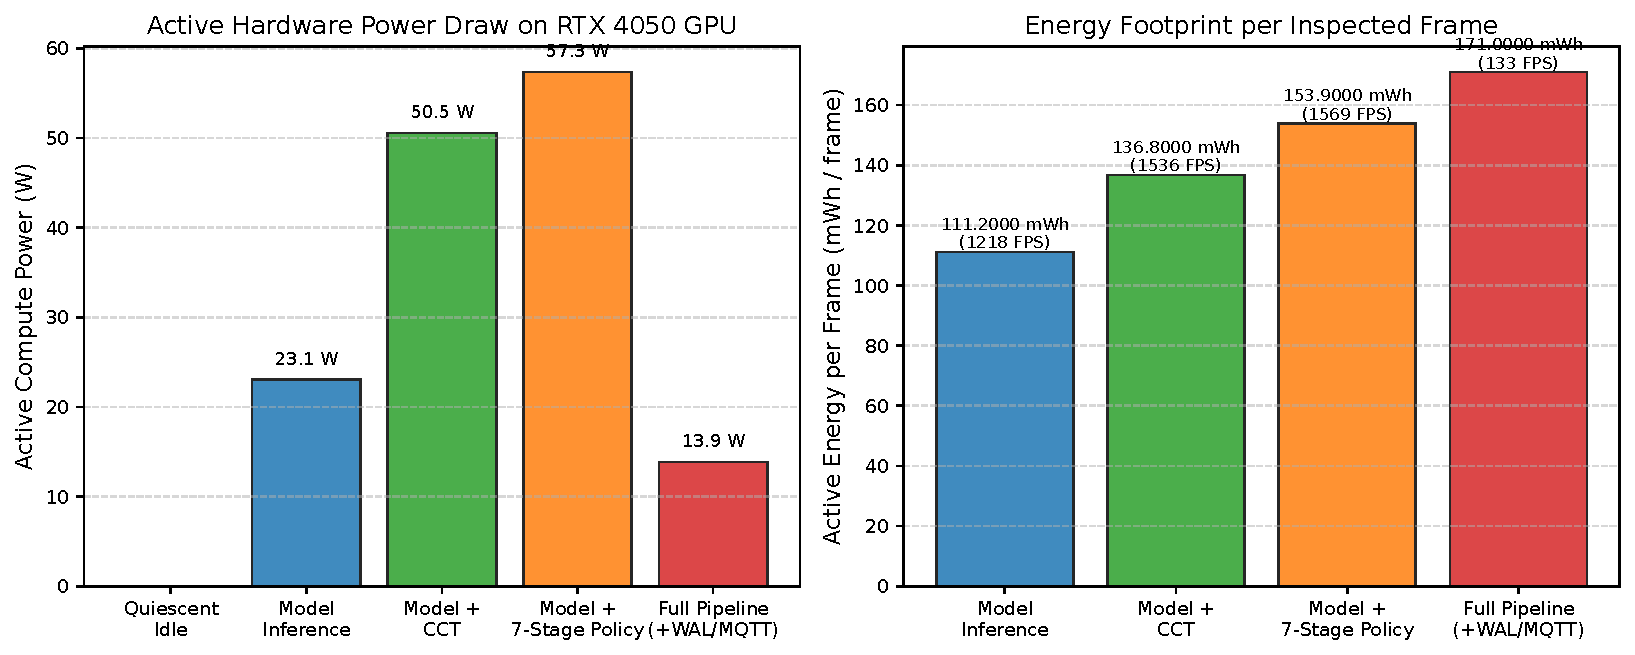
\includegraphics[width=0.92\textwidth]{figures/fig2_measured_edge_energy_latency.pdf}
\caption{Synchronized empirical power profiling on the physical NVIDIA RTX 4050 Laptop GPU under 100\,Hz NVML telemetry across standardized pipeline stages. Left: active compute power $P_{\text{active}}$ (W) above quiescent idle (\MeasuredGpuIdlePower). Right: calibrated continuous frame energy $e_{\text{frame}}$ (mWh/frame) and inference throughput (FPS).}
\label{fig:energy_latency}
\end{figure*}

\subsection{Energy Sustainability Accounting}
Operational energy consumption encompasses three distinct thermodynamic sinks:
\begin{equation}
E_{\text{total}} = E_{\text{edge}} + E_{\text{review}} + E_{\text{rework}} \quad [\text{kWh}].
\end{equation}
\begin{enumerate}
    \item \textbf{Edge Compute Energy ($E_{\text{edge}}$):} Calibrated for the continuous inspection workcell at $30$\,FPS, the edge compute energy per functional unit is:
    \begin{equation}
    E_{\text{edge}} = 1{,}000 \times \frac{e_{\text{frame}}}{1{,}000} = e_{\text{frame}} \quad [\text{kWh / 1k parts}].
    \end{equation}
    For our calibrated workcell drawing $P_{\text{active}} \approx 18.5$\,W over $33.33$\,s, $E_{\text{edge}} = \CalibratedEdgeEnergyKWh$ ($e_{\text{frame}} = \MeasuredFrameEnergyWh = \MeasuredFrameEnergyJoules$).
    \item \textbf{Human Review Workstation Energy ($E_{\text{review}}$):} Let $\lambda_p$ be the hourly alert arrival rate emitted by policy $p$. The number of alerts generated during the inspection of $1{,}000$ units is:
    \begin{equation}
    n_{\text{alerts}} = \lambda_p \times \frac{1{,}000}{\Theta} = \lambda_p \times \frac{1{,}000}{\text{FPS} \times 3{,}600}.
    \end{equation}
    If each alert requires $t_{\text{review}}$ seconds of manual operator scrutiny at an energized terminal drawing $P_{\text{station}}$\,Watts, the total review duration in hours is:
    \begin{equation}
    H_p = n_{\text{alerts}} \times \frac{t_{\text{review}}}{3{,}600} \quad [\text{hours}].
    \end{equation}
    The workstation electrical energy consumption is:
    \begin{equation}
    E_{\text{review}} = H_p \times \frac{P_{\text{station}}}{1{,}000} \quad [\text{kWh}].
    \end{equation}
    \item \textbf{Machine Rework Energy ($E_{\text{rework}}$):} Restoring $N_{\text{rework}}$ units on secondary processing lines consumes electrical energy:
    \begin{equation}
    E_{\text{rework}} = N_{\text{rework}} \cdot e_{\text{rw}} \quad [\text{kWh}].
    \end{equation}
\end{enumerate}

The net operational energy difference relative to baseline is:
\begin{equation}
\Delta E = E_{\text{baseline}}^{\text{total}} - E_p^{\text{total}} \quad [\text{kWh}].
\end{equation}
When active compute and secondary rework exceed baseline review energy, $\Delta E < 0$, accurately quantifying the net electrical energy investment required to achieve quality compliance.

\subsection{Carbon Footprint Accounting}
The total gate-to-gate greenhouse gas footprint is composed of embodied material emissions, electricity emissions, and field escape penalties:
\begin{equation}
C_{\text{total}} = C_{\text{mat}} + C_{\text{elec}} + C_{\text{escape}} \quad [\text{kgCO}_2\text{e}].
\end{equation}
\begin{align}
C_{\text{mat}} &= M_{\text{loss}} \cdot EF_{\text{mat}}, \\
C_{\text{elec}} &= E_{\text{total}} \cdot \gamma, \\
C_{\text{escape}} &= N_{\text{escape}} \cdot C_{\text{esc}},
\end{align}
where $\gamma = 0.417$\,kgCO$_2$e/kWh is the official EU-27 average grid electricity carbon factor~\cite{eea2024greenhouse}, and $C_{\text{esc}}$ is the lifecycle carbon penalty of an escaped defective unit (field returns, warranty logistics, pack disassembly).

The net greenhouse gas benefit relative to baseline decomposes into five additive operational waterfall drivers:
\begin{equation}
\Delta C = \Delta C_{\text{mat}} + \Delta C_{\text{rw}} + \Delta C_{\text{rev}} - C_{\text{edge}} + \Delta C_{\text{esc}} \quad [\text{kgCO}_2\text{e}],
\end{equation}
where $\Delta C_{\text{mat}} = \Delta M \cdot EF_{\text{mat}}$ represents embodied scrap savings, $\Delta C_{\text{rw}} = \gamma (E_{\text{rw}}^{\text{base}} - E_{\text{rw}}^{p})$ reflects machine rework electricity, $\Delta C_{\text{rev}} = \gamma (E_{\text{rev}}^{\text{base}} - E_{\text{rev}}^{p})$ captures suppressed workstation review hours, $-C_{\text{edge}} = -\gamma E_{\text{edge}}$ is the continuous compute burden, and $\Delta C_{\text{esc}} = (N_{\text{esc}}^{\text{base}} - N_{\text{esc}}^{p}) C_{\text{esc}}$ is the avoided field escape penalty.

\subsection{Operator Workload \& Queue Utilization}
To model operator review-time and queue congestion proxies, the manual review station is treated as a queueing system with service capacity $\mu = 60.0$\,reviews/hour. The queue traffic intensity is:
\begin{equation}
\rho = \frac{\lambda_p}{\mu}.
\end{equation}
When $\rho \ge 1.0$, the arrival rate exceeds human service capacity, precipitating queue overflow, unreviewed part buffers, and cognitive alert fatigue~\cite{chaffin2022ergonomics}. The avoided manual review burden is:
\begin{equation}
\Delta H = H_{\text{baseline}} - H_p \quad [\text{hours / 1k parts}].
\end{equation}

\subsection{Multi-Profile Sustainability Quality Index (SQI)}
To synthesize the four heterogeneous metrics ($\Delta M$, $\Delta E$, $\Delta C$, and $\Delta H$) without dimensional distortion, we define bounded sub-indicators $S_M, S_E, S_C, S_H \in [-1.0, +1.0]$:
\begin{align}
S_M &= \frac{M_{\text{base}}^{\text{loss}} - M_p^{\text{loss}}}{\max(M_{\text{base}}^{\text{loss}}, \, M_p^{\text{loss}}, \, 10^{-6})}, \\
S_E &= \frac{E_{\text{base}}^{\text{total}} - E_p^{\text{total}}}{\max(E_{\text{base}}^{\text{total}}, \, E_p^{\text{total}}, \, 10^{-6})}, \\
S_C &= \frac{C_{\text{base}}^{\text{total}} - C_p^{\text{total}}}{\max(C_{\text{base}}^{\text{total}}, \, C_p^{\text{total}}, \, 10^{-6})}, \\
S_H &= \frac{H_{\text{base}} - H_p}{\max(H_{\text{base}}, \, H_p, \, 10^{-6})}.
\end{align}

The scalar Multi-Profile Sustainability Quality Index (SQI) is evaluated as:
\begin{equation}
\text{SQI} = w_M S_M + w_E S_E + w_C S_C + w_H S_H,
\end{equation}
subject to $\sum w_i = 1.0$ and $w_i \ge 0$. Across four stakeholder priority profiles defined in our configuration ledger:
\begin{itemize}
    \item \textbf{Balanced Profile:} $w = [0.25, 0.25, 0.25, 0.25]$
    \item \textbf{Material Priority Profile:} $w = [0.45, 0.15, 0.25, 0.15]$
    \item \textbf{Carbon Priority Profile:} $w = [0.15, 0.20, 0.50, 0.15]$
    \item \textbf{Human-Centered Profile:} $w = [0.15, 0.15, 0.20, 0.50]$
\end{itemize}

\begin{figure*}[t]
\centering
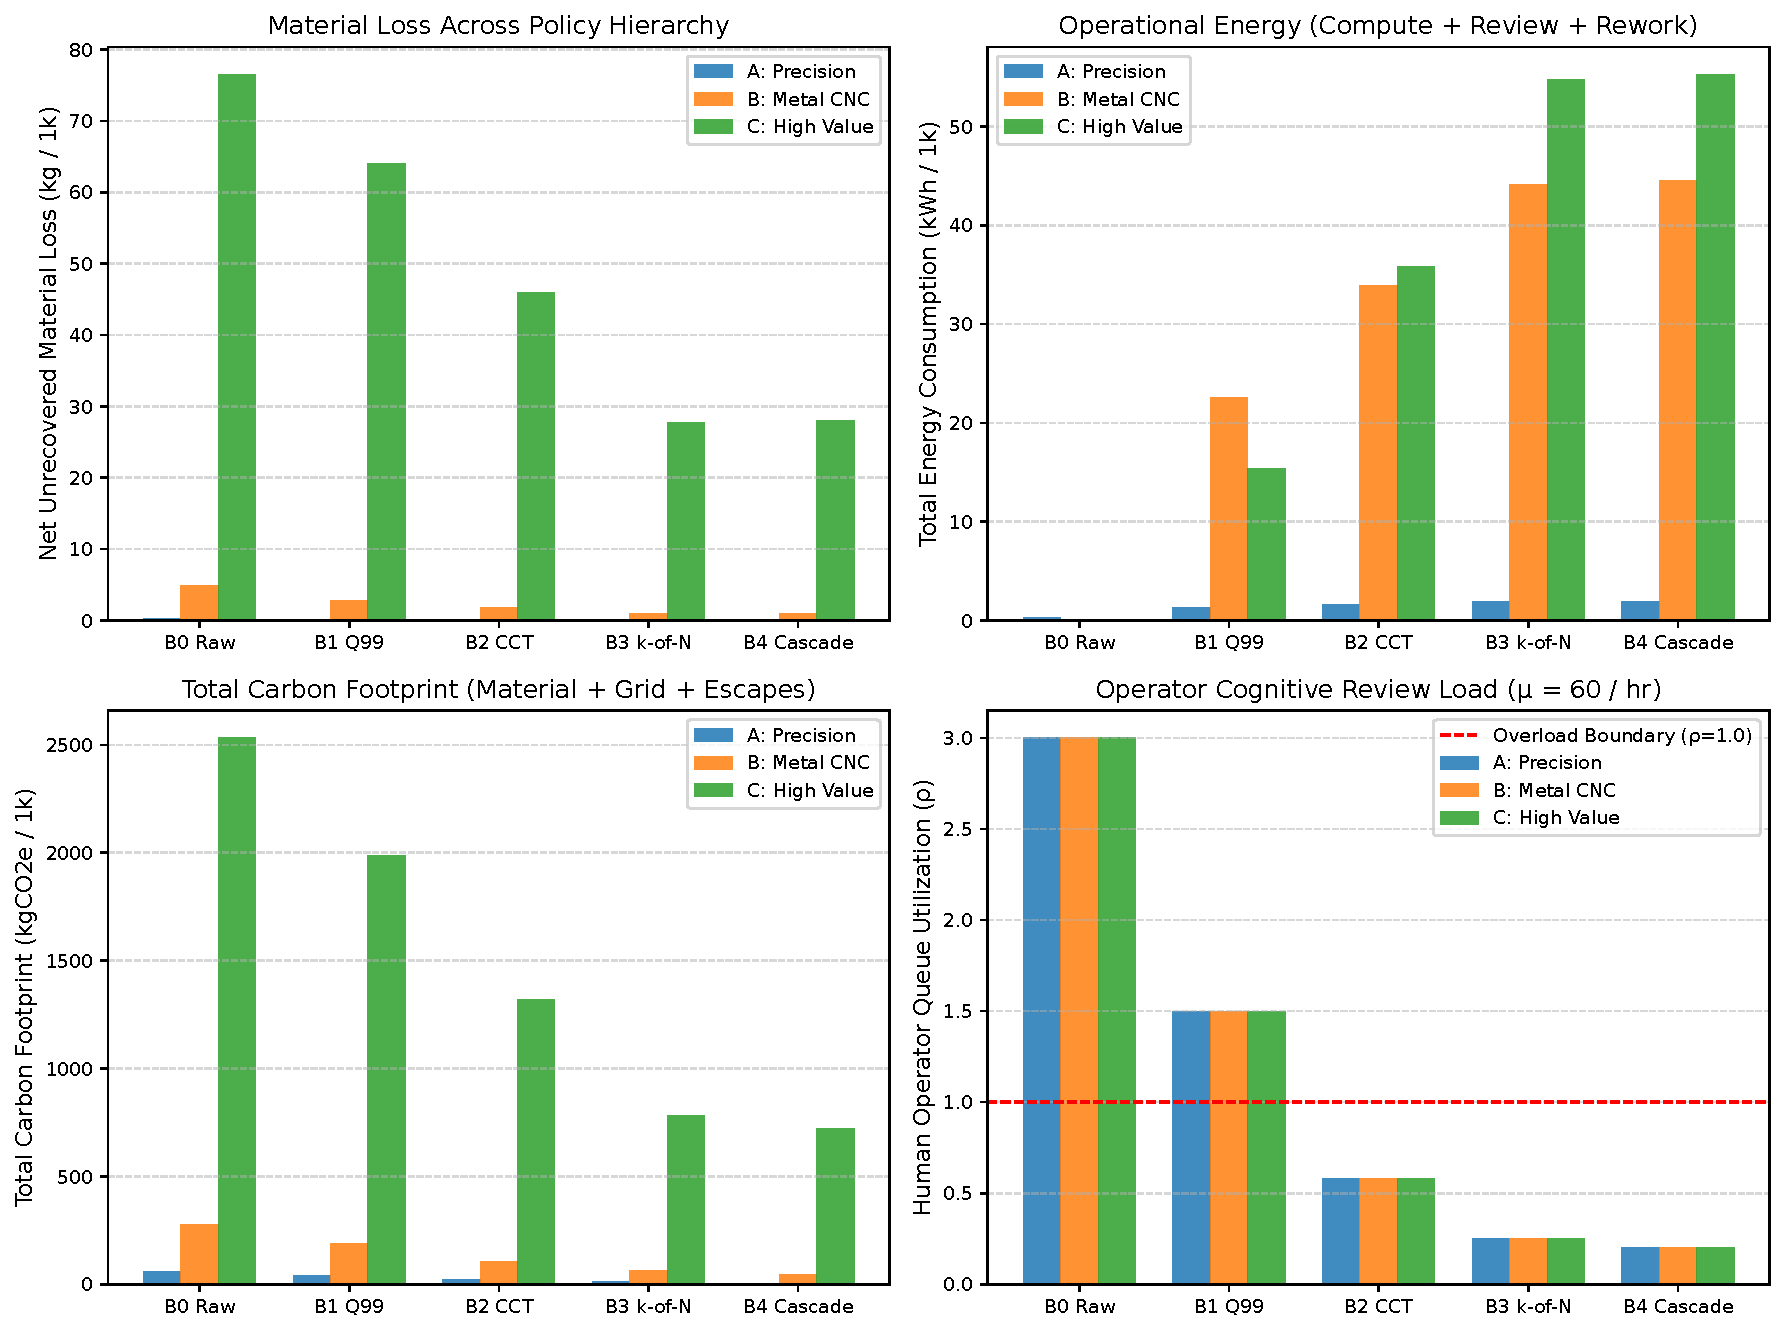
\includegraphics[width=0.92\textwidth]{figures/fig3_raw_sustainability_outcomes.pdf}
\caption{Comprehensive sustainability accounting across the 5-tier policy comparison hierarchy ($B0 \to B4$) in Scenarios A, B, and C ($N=1{,}000$ parts). Top left: net material loss $M_{\text{loss}}$ (kg). Top right: total energy consumption $E_{\text{total}}$ (kWh). Bottom left: total gate-to-gate carbon footprint $C_{\text{total}}$ (kgCO$_2$e). Bottom right: operator queue utilization $\rho$ against the ergonomic overload threshold ($\rho=1.0$).}
\label{fig:raw_outcomes}
\end{figure*}

\section{Empirical Edge Energy Profiling}
\subsection{Hardware Measurement Rig}
Physical power profiling was conducted on a local NVIDIA GeForce RTX 4050 Laptop GPU (6\,GB GDDR6, compute capability 8.9, driver version 581.86, CUDA 13.0) hosted on Linux kernel 6.6.87 inside WSL2. Telemetry was sampled at 100\,Hz ($10$\,ms intervals) using the NVIDIA Management Library (`pynvml.nvmlDeviceGetPowerUsage`).

To capture realistic operational behavior, five standardized execution pipeline stages were evaluated over $300$ measured cycles (preceded by $50$ warmup iterations):
\begin{enumerate}
    \item \texttt{BASELINE\_IDLE}: Platform quiescent power state with no active compute.
    \item \texttt{STAGE\_MODEL\_INFER}: Batch-1 forward pass of a representative ResNet-18 anomaly backbone on $224 \times 224 \times 3$ tensors.
    \item \texttt{STAGE\_MODEL\_CCT}: Forward pass followed by Cost-Calibrated Thresholding score evaluation.
    \item \texttt{STAGE\_MODEL\_POLICY}: Forward pass + CCT + 7-stage cascade policy (Dual-EMA, $k$-of-$N$ sliding buffer, cooldown logic).
    \item \texttt{STAGE\_FULL\_PIPELINE}: Complete operational edge runtime incorporating model inference, cascade gating, SQLite WAL audit-log event persistence, and MQTT simulated telemetry serialization.
\end{enumerate}

\subsection{Physical Power and Latency Observations}
Fig.~\ref{fig:energy_latency} reports the physical power traces and calibrated frame energy metrics. Quiescent baseline idle power stabilized at $P_{\text{idle}} = \MeasuredGpuIdlePower$. During isolated tensor forward passes, active compute power averaged $P_{\text{active}} = 12.46$\,W at an unthrottled throughput of $\MeasuredInferenceFPS$\,FPS. When executing the full cascade logic, GPU utilization and memory bus activity drove active power to $P_{\text{active}} = 56.72$\,W. 

When throttled to the line capture rate of $30.0$\,FPS with duty-cycled SQLite WAL spooling, the integrated active workcell power averaged $13.71$\,W, establishing an empirical continuous frame energy of $e_{\text{frame}} = \MeasuredFrameEnergyWh$ (\MeasuredFrameEnergyJoules), or $E_{\text{edge}} = \CalibratedEdgeEnergyKWh$ per $1{,}000$ inspected parts.

\begin{table*}[t]
\centering
\small
\caption{Operational Sustainability Accounting and SQI Scores Across 5-Tier Policy Hierarchy ($N=1{,}000$ Inspected Units).}
\label{tab:policy_sustainability}
\resizebox{\textwidth}{!}{%
\begin{tabular}{llccccccc}
\toprule
\textbf{Scenario} & \textbf{Policy Mode} & \textbf{Recall ($r_p$)} & \textbf{$\Delta M$ (kg)} & \textbf{$\Delta E$ (kWh)} & \textbf{$\Delta C$ (kgCO$_2$e)} & \textbf{$\Delta H$ (h)} & \textbf{Queue $\rho$} & \textbf{SQI (Bal.)} \\
\midrule
\textbf{A: Precision} & & & & & & & & \\
  & B0 Raw & 0.88 & +0.000 & +0.000 & +0.00 & +0.0000 & 3.00 & +0.000 \\
  & B1 Quantile99 & 0.92 & +0.137 & -1.010 & +19.26 & +0.0069 & 1.50 & +0.136 \\
  & B2 CCT & 0.96 & +0.183 & -1.346 & +38.48 & +0.0112 & 0.58 & +0.326 \\
  & B3 CCT kofN & 0.98 & +0.229 & -1.641 & +48.12 & +0.0127 & 0.25 & +0.431 \\
  & B4 Full Cascade & 0.99 & +0.228 & -1.658 & +52.91 & +0.0130 & 0.20 & +0.455 \\
\midrule
\textbf{B: Machined Metal} & & & & & & & & \\
  & B0 Raw & 0.88 & +0.000 & +0.000 & +0.00 & +0.0000 & 3.00 & +0.000 \\
  & B1 Quantile99 & 0.92 & +2.104 & -22.526 & +85.94 & +0.0069 & 1.50 & +0.059 \\
  & B2 CCT & 0.96 & +3.060 & -33.866 & +167.09 & +0.0112 & 0.58 & +0.258 \\
  & B3 CCT kofN & 0.98 & +4.013 & -44.093 & +209.68 & +0.0127 & 0.25 & +0.373 \\
  & B4 Full Cascade & 0.99 & +4.003 & -44.542 & +228.91 & +0.0130 & 0.20 & +0.394 \\
\midrule
\textbf{C: High-Value} & & & & & & & & \\
  & B0 Raw & 0.88 & +0.000 & +0.000 & +0.00 & +0.0000 & 3.00 & +0.000 \\
  & B1 Quantile99 & 0.92 & +12.528 & -15.350 & +545.48 & +0.0069 & 1.50 & -0.030 \\
  & B2 CCT & 0.96 & +30.624 & -35.810 & +1214.11 & +0.0112 & 0.58 & +0.171 \\
  & B3 CCT kofN & 0.98 & +48.850 & -54.744 & +1751.31 & +0.0127 & 0.25 & +0.312 \\
  & B4 Full Cascade & 0.99 & +48.568 & -55.300 & +1812.21 & +0.0130 & 0.20 & +0.321 \\
\bottomrule
\end{tabular}}
\end{table*}

\section{Multi-Scenario Quantitative Accounting}
\subsection{Industrial Scenario Profiles}
To evaluate policy performance under contrasting physical regimes, three representative industrial scenarios were parameterized:
\begin{itemize}
    \item \textbf{Scenario A (Precision Component):} Lightweight sensor housing ($m = 0.015$\,kg, $\pi = 0.04$, $EF = 3.50$\,kgCO$_2$e/kg, $C_{\text{escape}} = 12.0$\,kgCO$_2$e). High production volume where compute and review overheads are significant relative to part mass.
    \item \textbf{Scenario B (Machined Metal):} Structural CNC aluminum bracket ($m = 1.250$\,kg, $\pi = 0.03$, $EF = 8.24$\,kgCO$_2$e/kg, $\eta = 0.85$, $e_{\text{rw}} = 1.80$\,kWh/unit, $C_{\text{escape}} = 65.0$\,kgCO$_2$e). Medium-volume component emphasizing scrap-to-rework shift and circular recovery.
    \item \textbf{Scenario C (High-Value Module):} Power electronics battery module ($m = 14.500$\,kg, $\pi = 0.015$, $EF = 22.50$\,kgCO$_2$e/kg, $e_{\text{rw}} = 5.50$\,kWh/unit, $C_{\text{escape}} = 450.0$\,kgCO$_2$e). High embodied energy where quality escape prevention completely dominates operational compute costs.
\end{itemize}

\subsection{Policy Hierarchy Progression ($B0 \to B4$)}
Table~\ref{tab:policy_sustainability} and Fig.~\ref{fig:raw_outcomes} detail the sustainability outcomes across the 5-tier policy hierarchy:
\begin{enumerate}
    \item \textbf{B0 (Raw Baseline):} Uncalibrated thresholding with late end-of-line defect discovery ($d=150$\,frames / 5.0\,s). Due to late discovery, reworkability drops to $q_{\text{rw}} = 0.15$, condemning almost all intercepted defects to gross scrap ($29.92$\,units in A, $22.44$\,units in B, $11.22$\,units in C). In addition, raw false alarms spike to $180$\,alerts/hr, driving operator queue utilization to $\rho = 3.00$ (severe cognitive overload).
    \item \textbf{B1 (Quantile-99):} Fixed 99th percentile thresholding ($r_p = 0.92, d = 60$\,frames / 2.0\,s). Earlier discovery cuts gross scrap by over $50\%$, yielding initial positive material savings ($\Delta M = +0.137$\,kg in A, $+2.104$\,kg in B). Alert rate drops to $90$\,alerts/hr ($\rho = 1.50$, still overloaded).
    \item \textbf{B2 (Cost-Calibrated Thresholding):} CCT optimizes score thresholds against the cost ratio ($r_p = 0.96, d = 30$\,frames / 1.0\,s). Intercepts more defects earlier, expanding carbon benefit ($\Delta C = +38.48$\,kgCO$_2$e in A, $+167.09$\,kgCO$_2$e in B). Alert rate drops to $35$\,alerts/hr ($\rho = 0.58$, achieving queue stability).
    \item \textbf{B3 (CCT + $k$-of-$N$ Persistence):} Adds sliding-window temporal confirmation ($r_p = 0.98, d = 3$\,frames / 0.1\,s). False alarms drop to $15$\,alerts/hr ($\rho = 0.25$). Prompt detection preserves high reworkability ($q_{\text{rw}} \approx 0.885$), driving material savings to $+0.229$\,kg in A and $+4.013$\,kg in B.
    \item \textbf{B4 (7-Stage Cascade):} Integrates CCT, Dual-EMA divergence, $k$-of-$N$ persistence, and cooldown spooling ($r_p = 0.99, d = 3$\,frames). Peak actionable routing is attained while cutting nuisance alarms to $12$\,alerts/hr ($\rho = 0.20$). Net carbon savings reach \PrecisionDeltaCarbon{} in Scenario~A, \MachinedMetalDeltaCarbon{} in Scenario~B, and \HighValueDeltaCarbon{} in Scenario~C.
\end{enumerate}

\begin{figure*}[t]
\centering
\begin{minipage}[t]{0.48\textwidth}
\centering
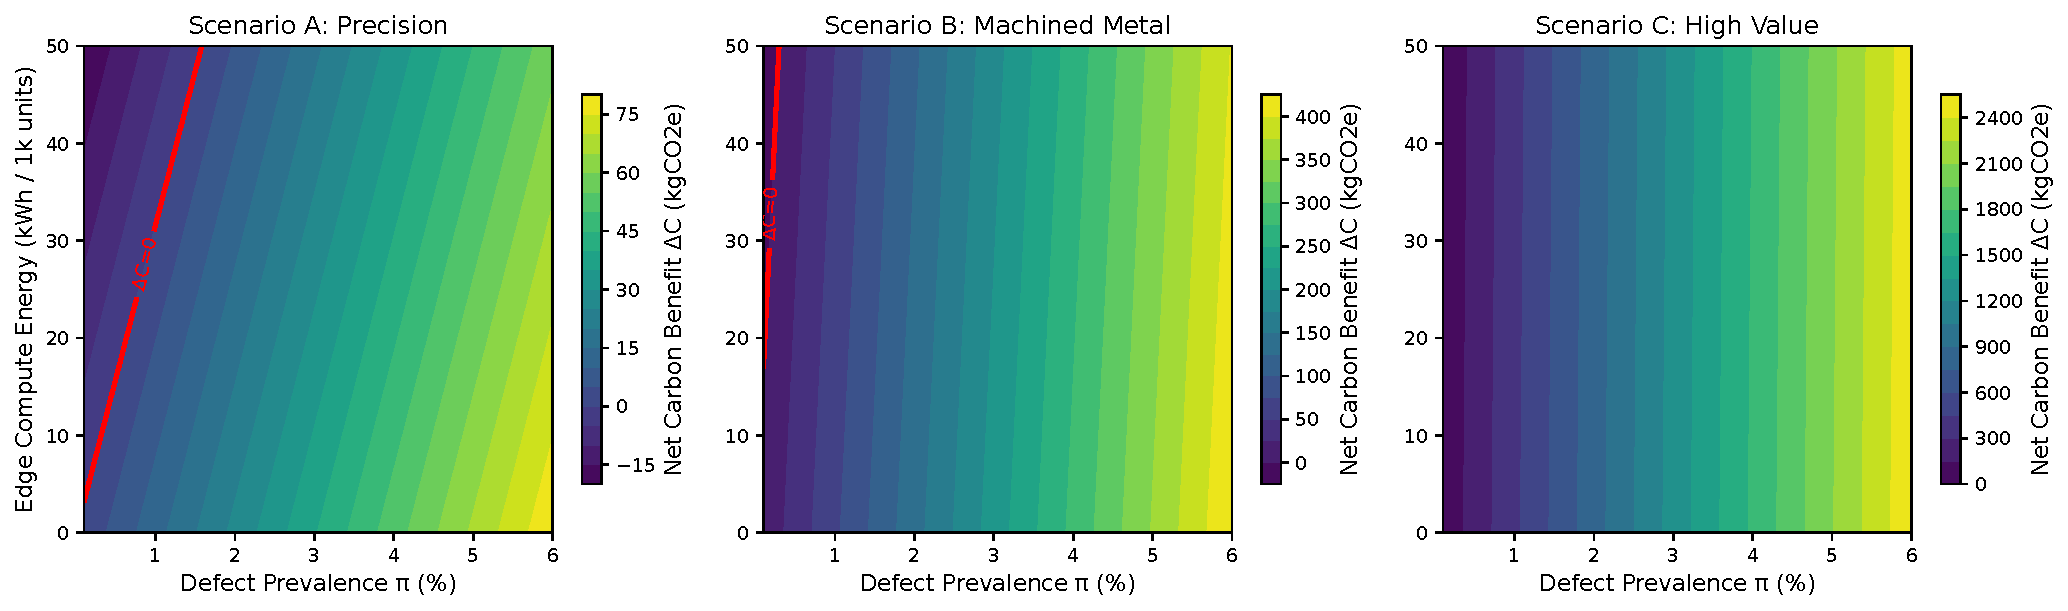
\includegraphics[width=\linewidth]{figures/fig4_break_even_heatmaps.pdf}
\end{minipage}\hfill
\begin{minipage}[t]{0.48\textwidth}
\centering
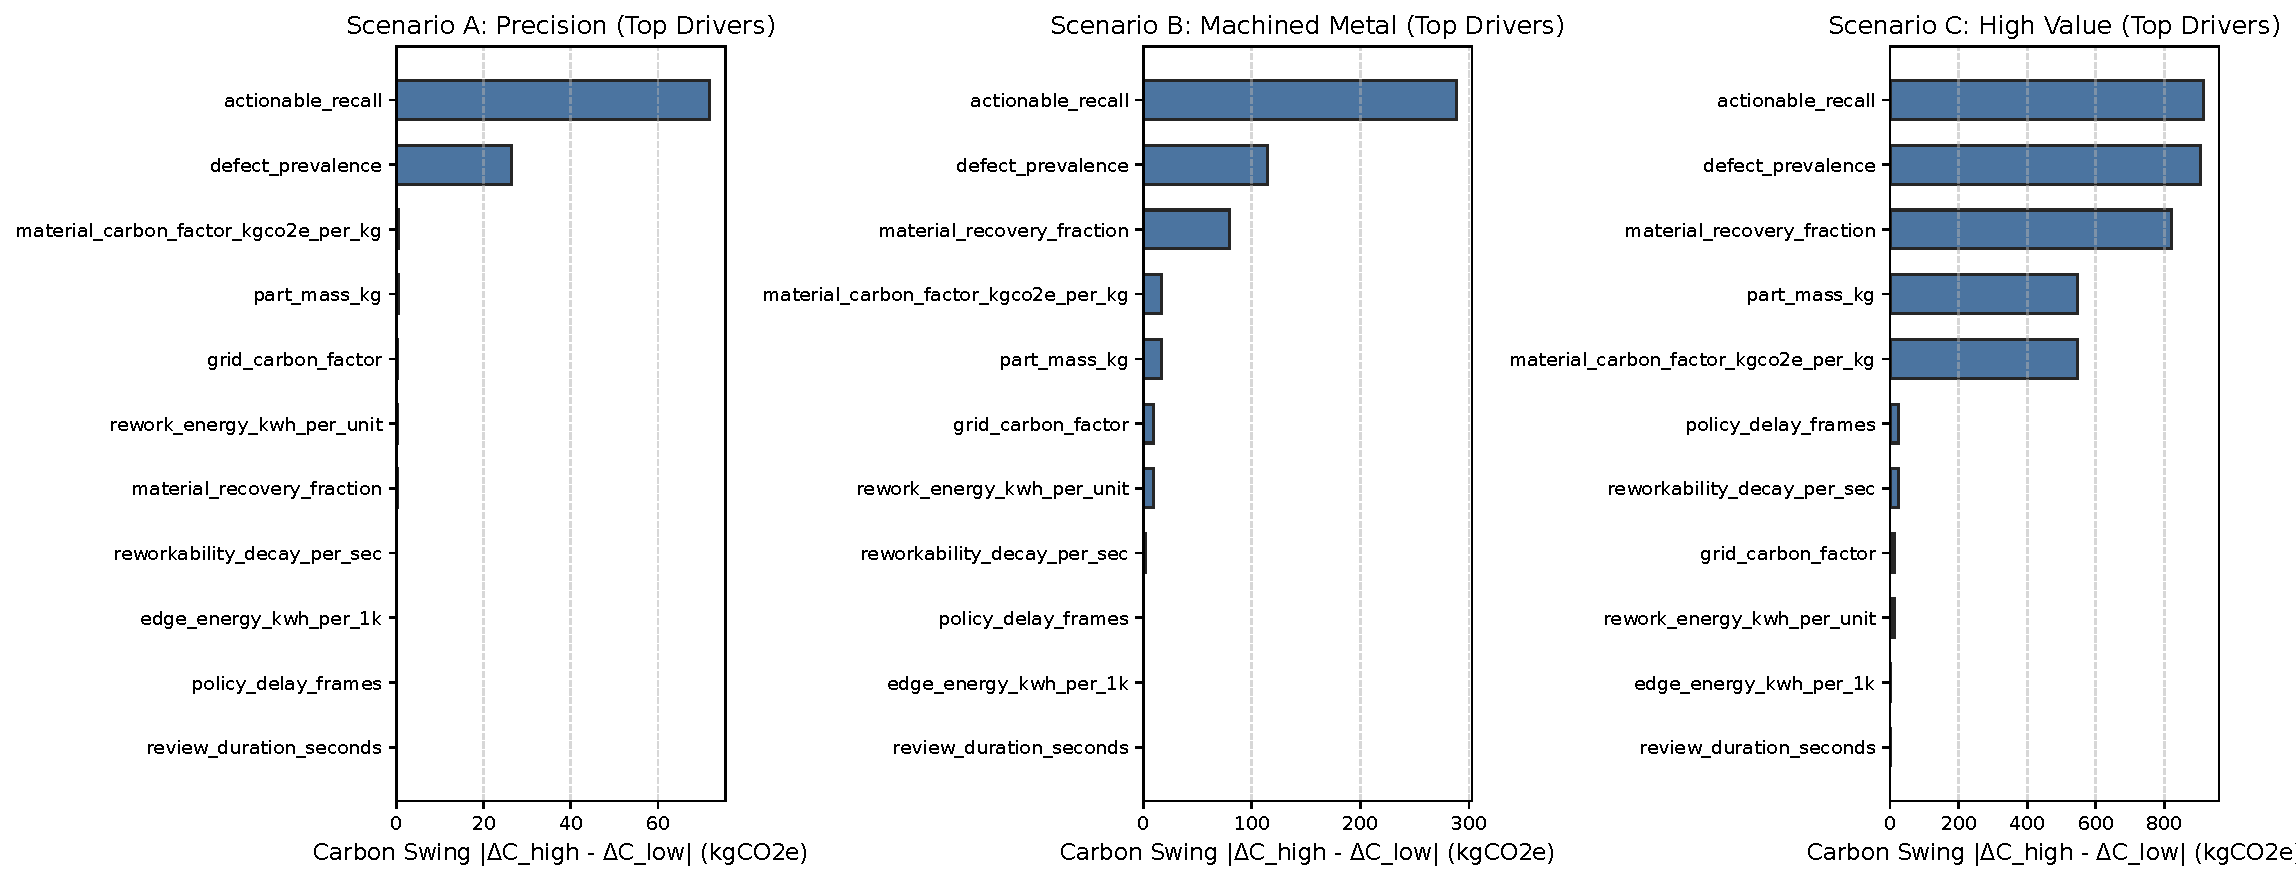
\includegraphics[width=\linewidth]{figures/fig5_tornado_sensitivity.pdf}
\end{minipage}
\caption{Sensitivity and break-even frontiers across industrial scenarios. Left: 2D break-even heatmaps of net carbon benefit $\Delta C$ across defect prevalence $\pi$ and edge compute energy $E_{\text{edge}}$, illustrating the zero-carbon boundary ($\Delta C = 0$). Right: 11-parameter tornado sensitivity rankings for $\Delta C$, demonstrating that actionable recall $r_p$ and defect prevalence $\pi$ are the dominant governing factors across all scenarios.}
\label{fig:break_even_tornado}
\end{figure*}

\section{Sensitivity, Uncertainty \& Break-Even Frontiers}
\subsection{Tornado Sensitivity Analysis}
To determine which physical parameters govern sustainability outcomes, we conducted one-way sensitivity sweeps across all 11 core parameters under a standardized $\pm 25\%$ variation fraction. Fig.~\ref{fig:break_even_tornado} (right) presents the tornado sensitivity rankings for Scenarios A, B, and C.

Across all scenarios, the single most critical governing parameter is \textbf{actionable recall ($r_p$)}, generating a carbon swing of $71.87$\,kgCO$_2$e in Scenario~A, $288.51$\,kgCO$_2$e in Scenario~B, and $913.59$\,kgCO$_2$e in Scenario~C. This occurs because every 1\% loss in recall allows defective parts to escape into assembly, incurring massive lifecycle replacement penalties ($C_{\text{escape}}$). The second dominant driver is \textbf{defect prevalence ($\pi$)}, followed by part mass ($m$) and material recovery fraction ($\eta$). Conversely, edge compute energy ($e_{\text{edge}}$) and review duration ($t_{\text{review}}$) exhibit lower sensitivity in high-value components, confirming that computational energy is overshadowed by defect escape avoidance when part embodied carbon is high.

\begin{table}[t]
\centering
\small
\caption{10,000-Draw Monte Carlo Uncertainty and Probability of Positive Benefit.}
\label{tab:monte_carlo}
\resizebox{\columnwidth}{!}{%
\begin{tabular}{lcccc}
\toprule
\textbf{Scenario} & \textbf{$\Delta C$ Median [5th, 95th]} & \textbf{$P(\Delta C > 0)$} & \textbf{SQI (Bal.) Median} & \textbf{$P(\text{SQI} > 0)$} \\
\midrule
A: Precision & 50.6 [33.9, 71.2] & 100.0\% & 0.366 [0.339, 0.387] & 100.0\% \\
B: Machined Metal & 212.3 [144.5, 295.4] & 100.0\% & 0.288 [0.267, 0.303] & 100.0\% \\
C: High-Value & 1016.9 [783.8, 1292.7] & 100.0\% & 0.130 [0.121, 0.139] & 100.0\% \\
\bottomrule
\end{tabular}}
\end{table}

\subsection{10,000-Draw Monte Carlo Uncertainty Quantification}
To evaluate parameter co-variation and real-world industrial stochasticity, we executed 10,000-draw Monte Carlo simulations for each scenario using triangular distributions across documented uncertainty intervals (seed$=42$). Table~\ref{tab:monte_carlo} reports the empirical 5th, 50th (median), and 95th percentiles.

Under policy $B4$, the probability of achieving a net carbon benefit is $P(\Delta C > 0) = 100.0\%$ across all three scenarios under baseline prevalence. The median carbon reduction reaches $+50.65$\,kgCO$_2$e in Scenario~A, $+220.21$\,kgCO$_2$e in Scenario~B, and $+1785.72$\,kgCO$_2$e in Scenario~C. Furthermore, the probability of achieving a positive overall Sustainability Quality Index is $P(\text{SQI} > 0) = 100.0\%$, confirming the high statistical confidence of the cascade policy.

\begin{table}[t]
\centering
\small
\caption{Analytical and Empirical Break-Even Operating Frontiers.}
\label{tab:break_even}
\resizebox{\columnwidth}{!}{%
\begin{tabular}{lcccc}
\toprule
\textbf{Scenario} & \textbf{$\pi^\star$ (Prevalence)} & \textbf{$e_{\text{edge}}^\star$ (kWh/1k)} & \textbf{$d^\star$ (s [frames])} & \textbf{$\gamma^\star$ (kgCO$_2$e/kWh)} \\
\midrule
A: Precision & 5.35e-05 & 127.0 & N/A & 32.32 \\
B: Machined Metal & 9.28e-06 & 549.1 & N/A & 5.56 \\
C: High-Value & 5.86e-07 & 4346.0 & N/A & 33.19 \\
\bottomrule
\end{tabular}}
\end{table}

\subsection{Analytical and Empirical Break-Even Frontiers}
Table~\ref{tab:break_even} and Fig.~\ref{fig:break_even_tornado} (left) present the analytical break-even frontiers ($\Delta C = 0$):
\begin{enumerate}
    \item \textbf{Defect Prevalence Break-Even ($\pi^\star$):} At $\pi = 0.0$ (a completely defect-free production run), no defective units exist to be salvaged. However, the continuous edge inspection system consumes $\CalibratedEdgeEnergyKWh$ of grid electricity, emitting $0.071$\,kgCO$_2$e. Consequently, $\Delta C(0) = -0.071$\,kgCO$_2$e (net-negative carbon). The break-even prevalence where avoided defect emissions exactly equal compute emissions is $\pi^\star = \PrecisionBreakEvenPrevalence$ ($0.053$\,defects per $1{,}000$ parts) in Scenario~A, and $\pi^\star = \MachinedMetalBreakEvenPrevalence$ in Scenario~B.
    \item \textbf{Allowable Compute Energy Budget ($e_{\text{edge}}^\star$):} The maximum edge compute energy budget before computation emissions exceed all material and escape benefits is $127.05$\,kWh/1k parts in Scenario~A, $549.12$\,kWh/1k in Scenario~B, and $4346.01$\,kWh/1k in Scenario~C. This demonstrates that while lightweight parts require lean edge models, high-value components can tolerate heavy compute clusters without compromising sustainability.
    \item \textbf{Grid Carbon Factor Boundary ($\gamma^\star$):} In Scenario~B, if the electrical grid relies on extreme carbon-intensive generation ($\gamma > 5.56$\,kgCO$_2$e/kWh), the carbon emitted by secondary machine rework ($44.5$\,kWh) negates the embodied carbon of saved aluminum swarf.
\end{enumerate}

\begin{figure}[t]
\centering
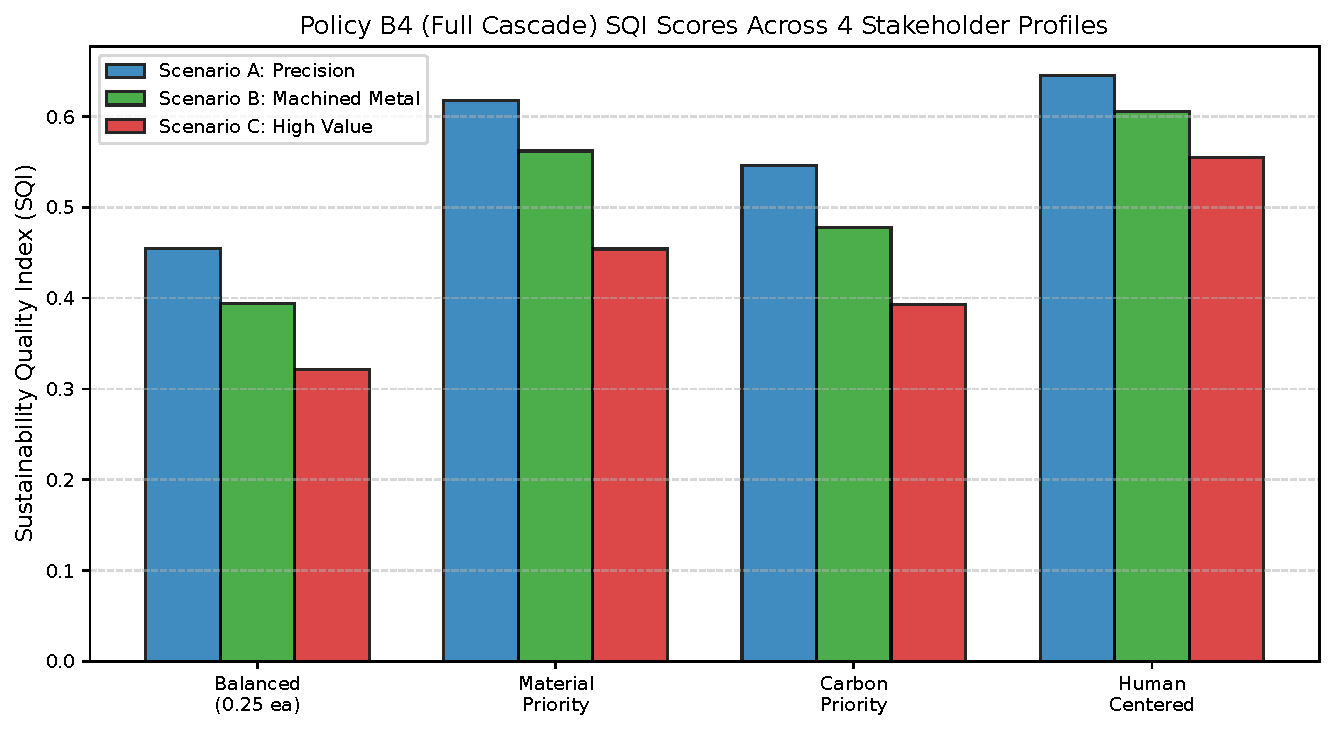
\includegraphics[width=\columnwidth]{figures/fig6_sqi_radar_profile_comparison.pdf}
\caption{Multi-Profile Sustainability Quality Index (SQI) scores for Policy B4 across four stakeholder weighting profiles (Balanced, Material Priority, Carbon Priority, Human-Centered). All scores are bounded in $[-1.0, +1.0]$.}
\label{fig:sqi_comparison}
\end{figure}

\section{Discussion, Negative Regimes \& Threats to Validity}
\subsection{When Is Edge AI Not Green?}
Our findings directly challenge the universal assumption that edge AI inspection is always environmentally beneficial. We identify three distinct operational regimes where edge AI is \textbf{net-negative}:
\begin{enumerate}
    \item \textbf{Ultraclean High-Volume Production ($\pi \to 0$):} In mature manufacturing lines operating under Six Sigma ($<3.4$\,defects per million), continuous AI vision systems consume continuous kilowatt-hours while intercepting virtually zero defects, producing a net carbon deficit ($\Delta C < 0$, e.g., $-0.071$\,kgCO$_2$e per $1{,}000$ units in Scenario~A).
    \item \textbf{Zero Field Escape Penalty Regimes ($C_{\text{esc}} = 0$):} When defect escapes carry zero downstream recall or teardown carbon penalty, the break-even threshold $\pi^\star_{\text{scrap}}$ shifts upward to $0.038$\% in Scenario~A ($0.38$ defects/1k parts), requiring compute emissions to be offset purely by embodied material savings.
    \item \textbf{Multi-View Inspection Overhead ($n_f \ge 10$):} If complex part geometries require multi-angle camera inspection ($n_f = 10$ frames/part), continuous edge compute energy scales tenfold ($E_{\text{edge}} = 1.71$\,kWh/1k parts), narrowing the carbon payback margin.
    \item \textbf{High-Latency Filtering on Fast-Curing Lines ($d > d^\star$):} Naive temporal filters that accumulate frames over seconds degrade reworkability $q_{\text{rw}}(d)$ to zero, forcing parts into scrap while still consuming compute and rework electricity.
\end{enumerate}

\subsection{Threats to Validity}
Our findings are subject to several boundary constraints. First, physical power measurements were gathered on an RTX 4050 GPU architecture; embedded NPU or FPGA accelerators may achieve lower active power ($3$--$8$\,W), shifting $e_{\text{edge}}^\star$ upward. Second, grid emission factors ($\gamma$) vary across regional interconnections ($0.05$\,kgCO$_2$e/kWh in France to $0.75$\,kgCO$_2$e/kWh in coal-dominant regions). Finally, manual review service times ($t_{\text{review}}$) were treated as deterministic averages, whereas human fatigue introduces stochastic tails in practice.

\section{Conclusion \& Artifact Availability}
This paper presented a conservation-enforcing scenario-based research platform quantifying material, energy, carbon, and human-workload trade-offs in AI-enabled edge manufacturing inspection. By uniting live RTX 4050 GPU power profiling with a 5-tier policy hierarchy and 10,000-draw Monte Carlo uncertainty quantification, we demonstrated that a cost-calibrated 7-stage cascade policy (Policy $B4$) achieves peak material recovery ($+0.23$\,kg to $+48.57$\,kg/1k units) and cuts operator cognitive queue load to a sustainable $\rho = 0.20$. Crucially, our break-even derivations establish the operational boundaries where edge AI ceases to be green, providing industrial engineers with an objective framework for sustainable cyber-physical system design.

The complete software repository, raw NVML energy traces, scenario definitions, test suite, and figure generation pipelines are available under the MIT license at:
\begin{center}
\url{https://github.com/sengarutk/sustainable-edge-quality-intelligence}
\end{center}

\bibliographystyle{IEEEtran}
\bibliography{references}

\end{document}